\vspace{0.5cm}
\noindent \lecture{5}{21/10/2021}

\section{Interazione con l'ambiente}

Consideriamo un qubit interagire con l'ambiente. Essendo il qubit un sistema non chiuso, non possiamo descrivere la sua evoluzione temporale come sola evoluzione del qubit. Bisognerà allora tenere in conto della sua interazione con l'ambiente e per farlo possiamo sfruttare la \textbf{matrice densità}. L'equazione del moto per la matrice densità, chiamata \textbf{equazione di Liouville-von Neumann}, segue direttamente dall'equazione di Schrödinger:
\begin{equation}
    \dv{\hat \rho}{t} = \sum_j \dv{t} \left(p_j\op{\psi_j}{\psi_j}\right)=\sum_j p_j\frac{1}{i\hbar}\left(\hat H \op{\psi_j}{\psi_j}-\op{\psi_j}{\psi_j}\hat H\right)=\frac{1}{i\hbar}\comm{\hat H}{\hat \rho} \, .
    \label{eq:liouville-von-neumann}
\end{equation}
L'evoluzione descritta dall'equazione \eqref{eq:liouville-von-neumann} è unitaria e la sua soluzione può essere scritta come
\begin{equation*}
    \hat \rho (t) = \hat U(t)\hat \rho(0) \hat U^\dagger(t) \, .
\end{equation*}
Tuttavia, questo processo descritto dalla \eqref{eq:liouville-von-neumann} non descrive alcun cambiamento sulla sua purezza, infatti quest'ultima risulta essere preservata:
\begin{equation*}
    \hat \xi(t) = \Tr\left(\hat \rho(t)^2\right) = \Tr\left(\hat U(t)\hat \rho(0) \hat U^\dagger(t)\hat U(t)\hat \rho(0) \hat U^\dagger(t)\right)=\Tr\left(\hat \rho (0)^2\right)=\hat \xi(0)
\end{equation*}
Questo significa che l'evoluzione di uno stato pure in una miscela di stati, includendo il processo di misurazione, non può essere descritto dalla \eqref{eq:liouville-von-neumann} ed è un processo essenzialmente non unitario.\\
Per risolvere questo aspetto l'hamiltoniana deve includere più termini
\begin{equation*}
    \hat H = \hat H_S + \hat H_E + \hat H_I \, ,
\end{equation*}
essi sono rispettivamente l'hamiltoniana di sistema, dell'ambiente e di interazione tra sistema e ambiente. Se assumiamo, come è ragionevole, che il sistema non abbia alcun effetto sull'ambiente e che l'hamiltoniana di interazione sia piccola (e quindi possiamo trattarla con la teoria perturbativa) possiamo facilmente studiare l'evoluzione della matrice densità nella rappresentazione d'interazione
\begin{equation*}
    \dv{\hat \rho_{int}}{t}=\frac{1}{i\hbar}\comm{\hat H_{int\,I}(t)}{\hat \rho_{int}(t)} \, ,
\end{equation*}
e
\begin{equation*}
    \hat \rho(t) = \hat \rho (-\infty) + \frac{1}{i\hbar}\int_{-\infty}^t \dd{t'}\comm{\hat H_{I}(t')}{\hat \rho(t')} \, ,
\end{equation*}
dove, supponendo che non solo inizialmente il sistema e l'ambiente fossero statisticamente indipendenti l'uno dall'altro, ma rimarranno tali, possiamo scrivere
\begin{align*}
    \hat \rho(-\infty) &= \hat \rho_S(-\infty)\otimes\hat\rho_E \\
    \hat \rho (t) &= \hat \rho_S(t)\otimes\hat\rho_E \, .
\end{align*}
A questo punto, possiamo tracciare la matrice densità sull'ambiente e ottenere una matrice densità ridotta per il sistema
\begin{equation*}
    \Tr_E\hat \rho(t) = \hat \rho_S(t)
\end{equation*}
Tornando alla rappresentazione di Schrödinger, svolgendo un paio di conti e assunzioni che non stiamo qui a discutere, otteniamo una \textbf{master equation} nella forma di \textbf{Lindblad}

\begin{equation}
    \dv{\hat\rho}{t} = \frac {1}{i\hbar} [\hat H, \hat \rho] + \sum_a \left( 2L_a \hat \rho L_a^\dagger - L_a^\dagger L_a\hat \rho - \hat \rho L_a^\dagger L_a\right)
    \label{eq:master}
\end{equation}
Cosa rende l'equazione \eqref{eq:master} così importante è il fatto che modelli l'evoluzione non unitaria della matrice densità del sistema. Lo stesso comportamento non potrebbe essere descritto dalla nostra equazione iniziale \eqref{eq:liouville-von-neumann} per l'intero insieme: sistema più ambiente.

\begin{esempio}[Evoluzione non unitaria di un qubit: rilassamento e sfasamento]
Supponiamo di considerare un sistema i cui stati siano $\ket 0$ e $\ket 1$. L'hamiltoniana di riferimento per questo sistema è
\begin{equation*}
    \hat H_S = \begin{pmatrix}E_0 & 0 \\ 0 & E_1\end{pmatrix}
\end{equation*}
Utilizzando la rappresentazione di interazione, possiamo scrivere la \textbf{master equation} come
\begin{equation}
        \dv{\hat\rho}{t} = \sum_a \left( 2L_a \hat \rho L_a^\dagger - L_a^\dagger L_a\hat \rho - \hat \rho L_a^\dagger L_a\right)
        \label{eq:master-example}
\end{equation}
a questo punto possiamo considerare i primi tre termini degli \textit{operatori di Lindblad}:
\begin{align*}
    & L_1 =L_1^\dagger =\sqrt \gamma \sigma_+\sigma_-=\sqrt\gamma\begin{pmatrix}1 & 0\\ 0 & 0\end{pmatrix}\\
    & L_2 = \sqrt{\frac{\Gamma}{2}}\sigma_- = \sqrt{\frac{\Gamma}{2}}\begin{pmatrix}0 & 0\\ 1 & 0\end{pmatrix} \\
    & L_2^\dagger = \sqrt{\frac{\Gamma}{2}}\sigma_+ = \sqrt{\frac{\Gamma}{2}}\begin{pmatrix}0 & 1\\ 0 & 0\end{pmatrix} \\
    & L_3 = \sqrt{\frac{\Gamma}{2}}\sigma_+ = \sqrt{\frac{\Gamma}{2}}\begin{pmatrix}0 & 1\\ 0 & 0\end{pmatrix} \\
    & L_3^\dagger = \sqrt{\frac{\Gamma}{2}}\sigma_- = \sqrt{\frac{\Gamma}{2}}\begin{pmatrix}0 & 0\\ 1 & 0\end{pmatrix}
\end{align*}
Sostituendo il primo in \eqref{eq:master-example} otteniamo
\begin{equation*}
    \dv{\hat\rho}{t} = \begin{pmatrix}0 & -\gamma\rho_{01}\\-\gamma\rho_{10} & 0\end{pmatrix}
\end{equation*}
che integrata
\begin{equation*}
    \hat \rho(t) = \begin{pmatrix}\rho_{00}(0) & \rho_{01}(0)e^{-\gamma t} \\ \rho_{10}(0)e^{-\gamma t} & \rho_{11}(0) \end{pmatrix}
\end{equation*}
I termini diagonali non vengono affatto modificati, quindi questa scelta di $L_1$ realizza quello che viene chiamato uno \textbf{sfasamento}. L'equazione ottenuta può essere considerata come un modello del processo di misura, in cui lo stato $\ket 0$ o $\ket 1$ del sistema è osservato, con $\tau_\gamma = 1/\gamma$ che fornisce il tasso di collasso dello stato.\\
Per quanto riguarda $L_2^\dagger$ ed $L_3$, otteniamo
\begin{equation*}
    \dv{\hat\rho}{t} = \begin{pmatrix}-\Gamma\rho_{00} & -(\Gamma/2)\rho_{01}\\-(\Gamma/2)\rho_{10} & \Gamma\rho_{00}\end{pmatrix}
\end{equation*}
con soluzione
\begin{equation*}
    \hat \rho(t) = \begin{pmatrix}\rho_{00}(0)e^{-\Gamma t} & \rho_{01}(0)e^{-(\Gamma/2)t} \\ \rho_{10}(0)e^{-(\Gamma/2) t} & 1-\rho_{00}(0)e^{-\Gamma t} \end{pmatrix}
\end{equation*}
e in maniera simile per $L_2$ e $L_3^\dagger$
\begin{equation*}
        \dv{\hat\rho}{t} = \begin{pmatrix} \Gamma\rho_{11} & -(\Gamma/2)\rho_{01}\\-(\Gamma/2)\rho_{10} & -\Gamma\rho_{11}\end{pmatrix}
\end{equation*}
con soluzione
\begin{equation*}
    \hat \rho(t) = \begin{pmatrix}1-\rho_{11}(0)e^{-\Gamma t} & \rho_{01}(0)e^{-(\Gamma/2)t} \\ \rho_{10}(0)e^{-(\Gamma/2) t} & \rho_{11}(0)e^{-\Gamma t} \end{pmatrix}
\end{equation*}
Oltre allo \textbf{sfasamento}, queste equazioni mostrano anche il \textbf{rilassamento} o \textbf{eccitamento} degli elementi diagonali. Fisicamente, ciò significa che Lindblads $L_2$, $L_3$ descrivono i processi concorrenti di trasmissione di energia tra il sistema e l'ambiente. Si noti che l'evoluzione delle matrici densità ricavate portano infine a uno stato puro, a un autostato dell'hamiltoniana del sistema. Affinché il sistema si rilassi in uno stato misto, l'equazione principale deve includere entrambi i termini che indicano uno \textbf{sfasamento} e un'\textbf{eccitazione} o \textbf{rilassamento}, con pesi appropriati. Se includiamo tutte gli operatori di Lindblad, la soluzione dell'equazione principale avrà la forma
\begin{equation*}
    \hat \rho(t) =
    \begin{pmatrix}
        \overline{\rho_{00}} + (\rho_{00}(0)-\overline{\rho_{00}})e^{-\Gamma t} & \overline{\rho_{01}}(0)e^{-(\Gamma/2+\gamma) t} \\
        \overline{\rho_{10}}(0)e^{-(\Gamma/2+\gamma) t} &
        \overline{\rho_{11}} + (\rho_{11}(0)-\overline{\rho_{11}})e^{-\Gamma t}
    \end{pmatrix}
\end{equation*}
dove i valori stazionari $\overline{\rho_{00}}+\overline{\rho_{11}}=\rho_{00}(0)+\rho_{11}(0)=1$ sono le eventuali probabilità di occupazione dei livelli. Se il sistema si rilassa verso l'equilibrio ad una certa temperatura, allora $\rho_{11}/\rho_{00} = \exp[-(E_1-E_0)/k_BT]$,
\end{esempio}
\noindent In questo contesto possiamo definire il \textbf{tempo di coerenza}, che risulta essere caratterizzato da:
\begin{itemize}
    \item \textbf{Relaxation time}: $\frac{1}{T_1}=\frac{\Gamma}{2}$
    \item \textbf{Dephasing time}: $\frac{1}{T_2}=\frac{\Gamma}{2} + \gamma$
\end{itemize}
Quando si realizza un qubit, è importante andare a misurare $T_1$ e $T_2$, così da caratterizzare al meglio il nostro sistema a due livelli.

\chapter{Misurazioni}
Abbiamo già introdotto il concetto di misura proiettiva e di misura a valori operatoriali positivi, ma avevamo sempre immaginato di agire su un grande insieme di stati uguali. Al contrario, adesso, ci concentreremo su misure di singoli oggetti, come può essere un qubit.
Lo strumento per misurare un singolo oggetto è, chiaramente, il fotone. Dal momento che esso può essere descritto sia come particella che come onda, più o meno localizzata, potremo studiarne la dispersione tramite il principio di indeterminazione di Heisenberg:

\begin{definizione}[\textbf{Principio di indeterminazione di Heisenberg}]
    Dati due osservabili $\hat A$ e $\hat B$, il valore d'aspettazione della deviazione standard degli stessi su di un particolare stato $\ket \psi$ è limitato dalla relazione:
    
    \begin{equation}
        \Delta A \Delta B \geq \frac{1}{2}\bra \psi \comm{A}{B} \ket \psi
    \end{equation}
\end{definizione}
\noindent Da questa equazione possiamo ricavare:
\begin{equation*}
    \Delta x \Delta p \geq \frac{\hbar}{2}
\end{equation*}
Spesso viene scritta e associata al principio di indeterminazione anche una \textbf{relazione di indeterminazione energia-tempo} che, tuttavia, non rientra nella casistica prevista dal principio di indeterminazione di Heisenberg (poiché non esiste alcun operatore "tempo").
\begin{equation*}
    \Delta E \Delta t \geq \frac{\hbar}{2}
\end{equation*}
Le relazioni che abbiamo scritto fino ad ora descrivono limiti intrinseci nella preparazione dei sistemi quantistici, ma sono chiaramente connessi a un'incertezza relativa alle misurazioni.
Vediamo ora un esempio per mostrare il collegamento fra incertezza nella preparazione e incertezza nella misura.

\section{Microscopio di Heisenberg}

\textbf{Microscopio di Heisenberg:}
Immaginiamo di avere un elettrone di cui vogliamo misurare la posizione. Abbiamo bisogno di almeno un fotone per visualizzare l'elettrone e dobbiamo fare in modo che esso sia deflesso dall'elettrone all'interno del cono ad angolo $\theta$ (in modo da incidere sulla lente del nostro microscopio).

\begin{wrapfigure}{r}{4cm}
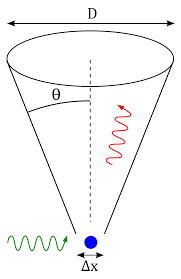
\includegraphics[width=3.5cm]{images/heisenberg_microscope.png}
\caption{Esperimento pensato del microscopio di Heisenberg.}\label{img-heisenberg_microscope}
\end{wrapfigure} 
\noindent A seconda dell'angolo di scattering dell'elettrone esso acquisirà un momento (più alta sarà l'energia del fotone più alto sarà il momento finale dell'elettrone).
Abbiamo quindi quella che viene chiamata \textbf{back action}: misurando un oggetto quantistico tramite un altro oggetto quantistico abbiamo influenzato e modificato il sistema stesso.
L'ottica classica ci fornisce una legge di diffrazione tale per cui:
\begin{equation*}
    \sin \theta \approx \frac{\lambda}{D}
\end{equation*}
Siccome il fotone è un'onda, il microscopio arriva a ottenere la posizione dell'elettrone con un'incertezza $\Delta x = \frac{\lambda}{\sin \theta}$ per cui si avrà:
\begin{equation*}
    -\frac{h}{\lambda}\sin \theta \le p_x \le \frac{h}{\lambda}\sin \theta
\end{equation*}
Da cui discende direttamente che: $\Delta p_x = \frac{2 h}{\lambda}\sin \theta$.
Dunque se voglio misurare solamente la posizione posso modificare $\lambda$ per avere una precisione arbitraria, ma non posso misurare in contemporanea il momento poiché:
\begin{equation*}
    \Delta p_x \Delta x = h
\end{equation*}
Che è una relazione evidentemente molto simile a quella ricavata dal principio di indeterminazione di Heisenberg: un'incertezza "alla Heisenberg" sulla sonda (il nostro fotone) ci porta a una necessaria incertezza sull'osservabile finale.